\documentclass{article}

\usepackage[margin=3cm]{geometry}

\usepackage{amsmath}
\usepackage{amssymb}
\usepackage{graphicx}
\graphicspath{ {./imgs/} }
\usepackage{mathtools}
\usepackage{dsfont}
\usepackage{graphicx}
\usepackage{tikz}
\usetikzlibrary{positioning}
\usepackage{csvsimple}
\usepackage{caption}
\usepackage{subcaption}
\usepackage{animate}
\usepackage{float}

\begin{document}


\title{Documentação \\
\large Algortimos II}
\author{Francisco Neves Tinoco Junior}
\maketitle

\newpage


\tableofcontents

\newpage


\section{Dataset} 

\subsection{Definição}

\paragraph{} Uma classe criada para automatizar e padrozinar a formatação do dataset.

\subsection{Funções}

	\begin{enumerate}
	
	\item[] \_\_init\_\_ : 
	
		\quad Resumo : Abre o arquivo .dat, coleta os pontos e aciona a função \_create\_dataset.
	
		\quad Entrada: 
	
			\qquad path : string -$>$ Caminho para o arquivo .dat
	
		\quad Pseudo Codigo
		
		\begin{enumerate}
	
		\item[.] Abra o arquivo e leia o seu valor
		\item[.] Separe as linhas pelo simbolo $@$, pois ele delimita as carecteristicas do dataset
		\item[.] Percora as linhas até achar uma que se inicie com data e save os valores dos pontos
		\item[.] Execute a função para criar o dataset (\_create\_dataset)
	
		\end{enumerate}
	
	\item[] \_create\_dataset: 
	
		\quad Resumo : Formata os valor dos pontos, transformar as categorias em numeros inteiros  e salva todos em uma numpy.array.
	
		\quad Pseudo Codigo :
		
		\begin{enumerate}
	
		\item[.] Percorar toda a listta de pontos salvos anteriormente. Para cada um dos pontos, passe os seus valores para o tipo float.
		\item[.] Crie um pandas.Dataframe com os pontos e as suas labels
		\item[.] Utilize a função pd.factorize para transformar os valores das labels em numericos
		\item[.] Save o valor dos pontos em uma numpy.array
	
		\end{enumerate}
	

\end{enumerate}

\subsection{Variaveis importantes}

\begin{enumerate}

\item[.] dataset : np.array -$>$ Conjunto de todos os pontos junto com o as suas classes. O ultimo valor de cada ponto é a sua classe
\item[.] indexador : dict -$>$ Indexa os numeros com as classes originais

\end{enumerate}



\section{KD} 

\subsection{Definição}

\paragraph{} Classe que implementa um arvore kd

\subsection{Funções}

	\begin{enumerate}
	
	\item[] \_\_init\_\_ : 
	
		\quad Resumo : Utilize a função make\_kd para fazer uma kdtree e salva na variavel $kd\_tree$
	
		\quad Entrada: 
	
			\qquad data : np.array -$>$ conjunto de pontos criado pela classe Dataset
	
		\quad Pseudo Codigo
		
		\begin{enumerate}
	
		\item[.]Utilize a função make\_kd utilizando data com entrada para fazer uma kdtree e salva na variavel $kd\_tree$
	
		\end{enumerate}
	
	\item[] create\_node: 
	
		\quad Resumo : Cria o nó de uma arvore.
	
		\quad Pseudo Codigo :
		
		\begin{enumerate}
	
		\item[.] Retorne um nó
	
		\end{enumerate}

		\quad Propriedades do nó:

		\begin{enumerate}
	
		\item[.] CORTE : int -$>$ O valor que divide a arvore. Caso None, indica que o nó é uma folha da arvore
		\item[.] DIM : int -$>$ Indica a diminsão que o valor de corte se refere. É igual a Deep mod Dim, aonde Deep é a profundidade da arvore e dim é a quantidade de dimensões dos pontos
		\item[.] POINT : list -$>$ Indica o valor do ponto. Sse len(POINT) == 0, então o nó não é uma folha
		\item[.] MENOR: dict -$>$ Arvore da esquerda com os valores menores que CORTE
		\item[.] MAIOR: dict -$>$ Arvore da direita com os valores maiores ou iguais que CORTE

		\end{enumerate}
		
		\quad Notas:

		\begin{enumerate}
	
		\item[.] A propriedade isinstance(tree["CORTE"], type(None)), i.e., caso tree["CORTE"] == None, vai ser usado para conferir se a arvore é uma folha
		\item[.] Essa função foi criada para criar um padrão de representação entre os nós da arvore

		\end{enumerate}

	\item[] insert\_kd: 
	
		\quad Resumo : Insere um nó com o valor de $point$ na arvore.

		\quad Entrada: 
	
			\qquad tree :dict -$>$ Arvore em que $point$ tem que ser inserida
			
			\qquad point : np.array -$>$ Ponto a ser inserido

			\qquad n\_dim : int -$>$  O numero de dimensões de $point$
	
		\quad Pseudo Codigo :
		
		\begin{enumerate}
	
		\item[.] Teste se a arvore é uma folha ou não.

		\item[.] Caso seja.
			\begin{enumerate}
			\item[.] Retire o ponto presente em tree["POINT"] e save ele em $p0$. Altere o valor de tree["POINT"] para None.
			\item[.] Crie dois novos nós, l\_tree e r\_tree, e atualize os seus valores de DIM para ((dim + 1) mod n\_dim ), sendo dim a dimensão de $tree$
			\item[.] Confere o valor de $p0$ e $point$ em relação a dim. Caso $p0 < point$, coloque $p0$ em l\_tree e $point$ em r\_tree. Se não, faça o contrario.
			\item[.] Use a mediana do valor de $p0$ e $point$ em dim para definir o valor de Corte de tree
			\item[.] Adicione l\_tree na arvore MENOR de tree e r\_tree na arvore MAIOR de tree   
			\end{enumerate}

		\item[.] Se não for:
		
			\begin{enumerate}
			\item[.] Veja se o valor da dimensão do ponto é menor ou não ao corte. Se for, repita insert\_kd só que com tree = tree["MENOR"]. Se não,  repita insert\_kd só que com tree = tree["MAIOR"].
			\end{enumerate}
	
		\end{enumerate}
		
		\quad Notas:

		\begin{enumerate}
	
		\item[.] insert\_kd foi implementada de maneira recursiva.

		\end{enumerate}

	\item[] make\_kd: 
	
		\quad Resumo : Cria um arvore kd com todos os dados presentes em $data$

		\quad Entrada: 
	
			\qquad data : np.array -$>$ conjunto de pontos criado pela classe Dataset
	
		\quad Pseudo Codigo :
		
		\begin{enumerate}
	
		\item[.] Cria um nó $kd\_tree$ que contem o primeiro valor de data e DIM = 0.

		\item[.] Usando a função $insert\_kd$, insira todos os pontos restantes de data em $kd\_tree$

		\item[.] Retorne $kd\_tree$
		\end{enumerate}	

\end{enumerate}

\subsection{Variaveis importantes}

\begin{enumerate}

\item[.] kd\_tree : dict -$>$ Arvore kd criada usando os pontos presentes em data

\end{enumerate}


\section{X\_nn} 

\subsection{Definição}

\paragraph{} Classe que representa um modelo de classificação kneighbors

\subsection{Funções}

	\begin{enumerate}
	
	\item[] fit : 
	
		\quad Resumo : Função que separa os conjuntos de treino e teste gerados por $Dataset$ e cria a arvore kd a partir da classe $KD$
	
		\quad Entrada: 
	
			\qquad path : string -$>$ Diretorio aonde está o dataset

			\qquad test\_size : int, default = 0.3 -$>$ Proporção do conjunto de teste em relação à todos od dados
	
		\quad Pseudo Codigo:
		
		\begin{enumerate}
	
		\item[.] Utilizando $path$ como entrada em $Dataset$, formate os dados e save em data
		\item[.] Utilizando o valor de $test\_size$, separe os dados em 
		
			\begin{enumerate}
			\item[.] X\_train : numpy.array -$>$ Conjunto de treinamento contedo os pontos
			\item[.] y\_train : numpy.array -$>$ Conjunto de treinamento contendo as labels
			\item[.] X\_train : numpy.array -$>$ Conjunto de teste contedo os pontos
			\item[.] y\_train : numpy.array -$>$ Conjunto de teste contendo as labels			
			\end{enumerate}

		\item[.] Utilizando $X\_train$ como entrada, monte uma arvore kd com a classe $KD$
	
		\end{enumerate}
	
	\item[] knn: 
	
		\quad Resumo : Função que encontra os $k\_size$ pontos mais proximos de todos os ponto em $X\_test$.

		\quad Entrada: 
	
			\qquad k\_size : int -$>$ Numero de pontos a serem preditos

			\qquad cpu : int, default = -1 -$>$ Numero de cpus para serem usadas, Caso -1, usa todas
	
		\quad Pseudo Codigo:
		
		\begin{enumerate}
	
		\item[.] Para cada ponto presente $X\_test$, utilize a função $multi\_knn$ para calcular os $k\_size$ pontos mais proximos. Guarde todas as pevisões em $predict$.
		\item[.] Retorne predicts
	
		\end{enumerate}

	\item[] multi\_knn: 
	
		\quad Resumo : Função intermediaria para ser possivel utilizar o multiprocessing.

		\quad Entrada: 
	
			\qquad point : np.array -$>$ Ponto para ser encontra os k\_size pontos mais proximos
	
		\quad Pseudo Codigo :
		
		\begin{enumerate}
	
		\item[.] Utilizando a função $knn\_aux$, calcule os $k\_size$ pontos mais proximos de $point$. Salve o resultado em $kneighbor$.
		\item[.] Retorne kneighbor

		\end{enumerate}

	\item[] knn\_aux: 
	
		\quad Resumo : Função que localiza os $k\_size$ mais proximos de point

		\quad Entrada: 
	
			\qquad tree : dic -$>$ Arvore em que sera realizada a busca

			\qquad point : np.array -$>$ Ponto para ser encontra os k\_size pontos mais proximos

			\qquad k\_size : int -$>$ Numero de neighbors a serem localidados

			\qquad kneighbor : list -$>$ Pontos mais proximos

			\qquad maior\_distancia : list-$>$ Maior distancia do ponto mais longe de point em kneighbor e a sua posição

			\qquad check : list -$>$ Numero de pontos testados pelo algoritmo

			\qquad dists : list -$>$ Lista com as distancias entre o kneighbor e point
	
		\quad Pseudo Codigo:
		
		\begin{enumerate}
	
		\item[.] Teste se $tree$ é uma folha
		
		\item[.] Se for:

			\begin{enumerate}
			\item[.] Teste se o numero de pontos em $kneighbor$ já atingiu o maximo ($k\_size$).
			
			\item[.] Se atingiu:
				\begin{enumerate}
				\item[.] Teste se a distancia do novo ponto a $point$ dist é menor que a maior distancia no momento.

				\item[.] Se for:

					\quad Troque o ponto mais longe com esse novo ponto em $kneighbor$, assim como a suas distancias em $dists$.

					\quad Calcule o novo ponto mais longe assim como a sua distacia e salve esses dados em $maior\_distancia[1]$.
					
				
				\end{enumerate}

			\item[.] Se não atingiu:
				\begin{enumerate}
				\item[.] Adicione o ponto a $kneighbor$.
				\item[.] Se a distacia de $point$ ao novo ponto $dist$ for a maior, defina $maior\_distancia[0]$ = dist e $maior\_distancia[1]$ = len(kneighbor) - 1, i.e., salve a nova maior distancia e a posição do ponto na lista
				\item[.] Adicione dist a $dists$.				
				\end{enumerate}

			\end{enumerate}
		


		\item[.] Se não for:
			
			\begin{enumerate}
			\item[.] Seja dif a diferença entre o $point$ e corte.
			\item[.] Caso ainda não tenha atingido o limite de pontos ou dif seja menor que a maior distancia, continue procurando nas arvores $MENOR$ e $MAIOR$
			\item[.] Se não, confira em qual arvore o ponto entraria pelo $CORTE$ e continue a busca somente nela.

			\end{enumerate}
		
	
		\end{enumerate}
		
		\quad Notas:

		\begin{enumerate}
	
		\item[.] As variaveis $maior\_distancia$ e $dists$ são usadas para evitar ter que ficar recalculado as distancias entre $point$ e os pontos em $kneighbor$ 

		\end{enumerate}

	\item[] define\_class: 
	
		\quad Resumo : Função que classifica a classe considerando os kneighbors

		\quad Entrada: 
	
			\qquad kneighbors : list -$>$  Lista contendo k\_size neighbors para um ponto
	
		\quad Pseudo Codigo :
		
		\begin{enumerate}
	
		\item[.] Para cada ponto n em kneighbors, procure em $y\_train$ qual a sua classe.
		\item[.] Retorne a classe com mais pontos. Em caso de empate, retorne aleatoriamente uma das classes com mais pontos.
	
		\end{enumerate}
		
		\quad Notas A escrever:

		\begin{enumerate}
	
		\item[.] É necessario compara n aos pontos em $X\_train$ para saber qual é a sua posição e, sucecivamente, a sua classe.

		\end{enumerate}

	\item[] predict: 
	
		\quad Resumo : Função que prediz a classe de todos os valores em $X\_test$

		\quad Entrada: 
	
			\qquad k\_size : int -$>$ Numero de pontos a serem preditos.
	
			\qquad cpu : int, default = -1 -$>$ Numero de cpus para serem usadas, Caso -1, usa todas
	
		\quad Pseudo Codigo A escrever :
		
		\begin{enumerate}
	
		\item[.] Utilizando a função $knn$, predica os $k\_size$ vizinhos de cada ponto contido em $X\_test$ e guarde em $pred$
		\item[.] Utilizado define\_class, predica a classe de cada ponto i com os vizinhos $pred[i]$. Armazene as classes previstas em $classes\_pred$
		\item[.] Retorne $classes\_pred$ 
	
		\end{enumerate}

	\item[] evaluate: 
	
		\quad Resumo : Função que calcula as metricas de acerto.

		\quad Entrada: 
	
			\qquad k\_size : int -$>$ Numero de pontos a serem preditos.
	
			\qquad cpu : int, default = -1 -$>$ Numero de cpus para serem usadas, Caso -1, usa todas
	
	
		\quad Pseudo Codigo A escrever :
		
		\begin{enumerate}
	
		\item[.] Utilizando predict, pege cada classe prevista para cada ponto em $X\_test$.
		\item[.] Calcule qual é classe c com mais pontos no conjuto de teste.
		\item[.] Usando $evaluate\_aux$, os valores de true\_positives(tp), true\_negatives(tn), false\_positives(fp) e false\_negatives(fn)
		\item[.] Retorne as metricas de acuracia, precição e revocação.
	
		\end{enumerate}

	\item[] evaluate\_aux: 
	
		\quad Resumo : Função que calcula as metricas de acerto.

		\quad Entrada: 
	
			\qquad c : int -$>$ Classe tomada como padrão

			\qquad pred : list -$>$ Classes previstas para os pontos
	
		\quad Pseudo Codigo :
		
		\begin{enumerate}
	
		\item[.] Considerando $c$ como a classe referencial, calcule os  true\_positives(tp), true\_negatives(tn), false\_positives(fp) e false\_negatives(fp) de $pred$ em relação a $y\_test$
		\item[.] Retorne tp,tn,fp,fn
	
		\end{enumerate}


\end{enumerate}

\subsection{Variaveis importantes}

\begin{enumerate}
\item[.] X\_train : np.array -$>$ Contem os dados de treinamento
\item[.] y\_train : np.array -$>$ Contem a label dos dados de treinamento
\item[.] X\_test : np.array   -$>$  Contem os dados de teste
\item[.] y\_test : np.array   -$>$  Contem a label dos dados de teste
\item[.] kd\_tree : dict -$>$  Uma kd\_tree criada a partir dos dados de treinamento
\end{enumerate}

\subsection{Notas}

\begin{enumerate}
\item[.] A classe foi criada em cima de calcularas metricas e predições do dataset passado em $path$. Logo, utiliza-la para tentar prever pontos fora do arquivo não é possivel.
\end{enumerate}

\section{Resultado do modelo}

\paragraph{} A fim de testar como o modelo estava se comportando, foram escolhidos doze datasets que continham um conjunto de pontos e a suas labels. Foi-se aplicado o X\_nn em cada um dos datasets variando a quantidade de vizinhos a serem considerados na classificação. 
 
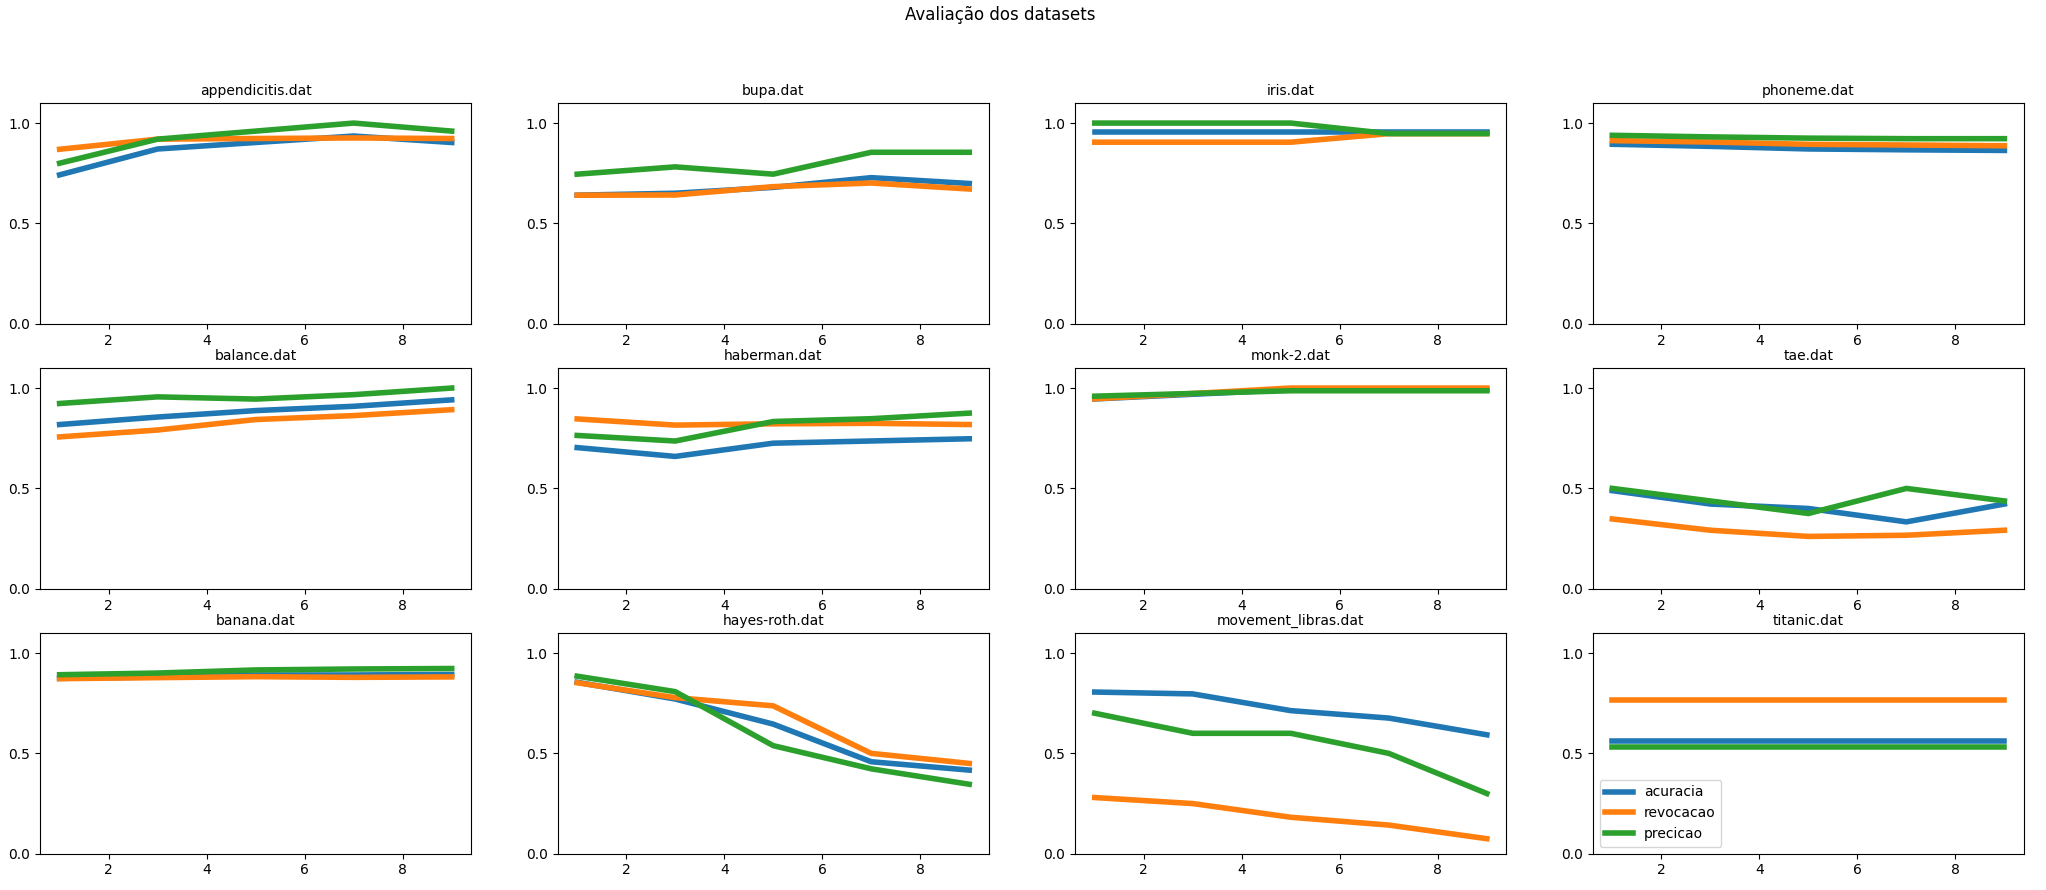
\includegraphics[width=\textwidth]{datasets.png}

O grafico acima demonstra os resultados para cada um dos datasets. É possivel observar que o algoritmo teve um resultado possitivo na classificação da maioria dos datasets, sendo que o aumento do numero de vizinhos influenciava as taxas de acertos, via de regra positivamente. Nos datasets em que o resultado
foi misto ou ruim, é possivel ver uma relação inversa, aonde o aumento do numero de vizinhos acabava prejudicando os resultados. Essa oscilação de resultados pode ser resultante de diversos fatores, desde falhas na implementação, até a separação de alguns datasets não se muito linear, necessitando de se aplicar
algumas tecnicas, como aplicar um kernel, antes de se utilizar o algoritmo. Todas as metricas acabaram tendo uma flutuação bastante parecida. 

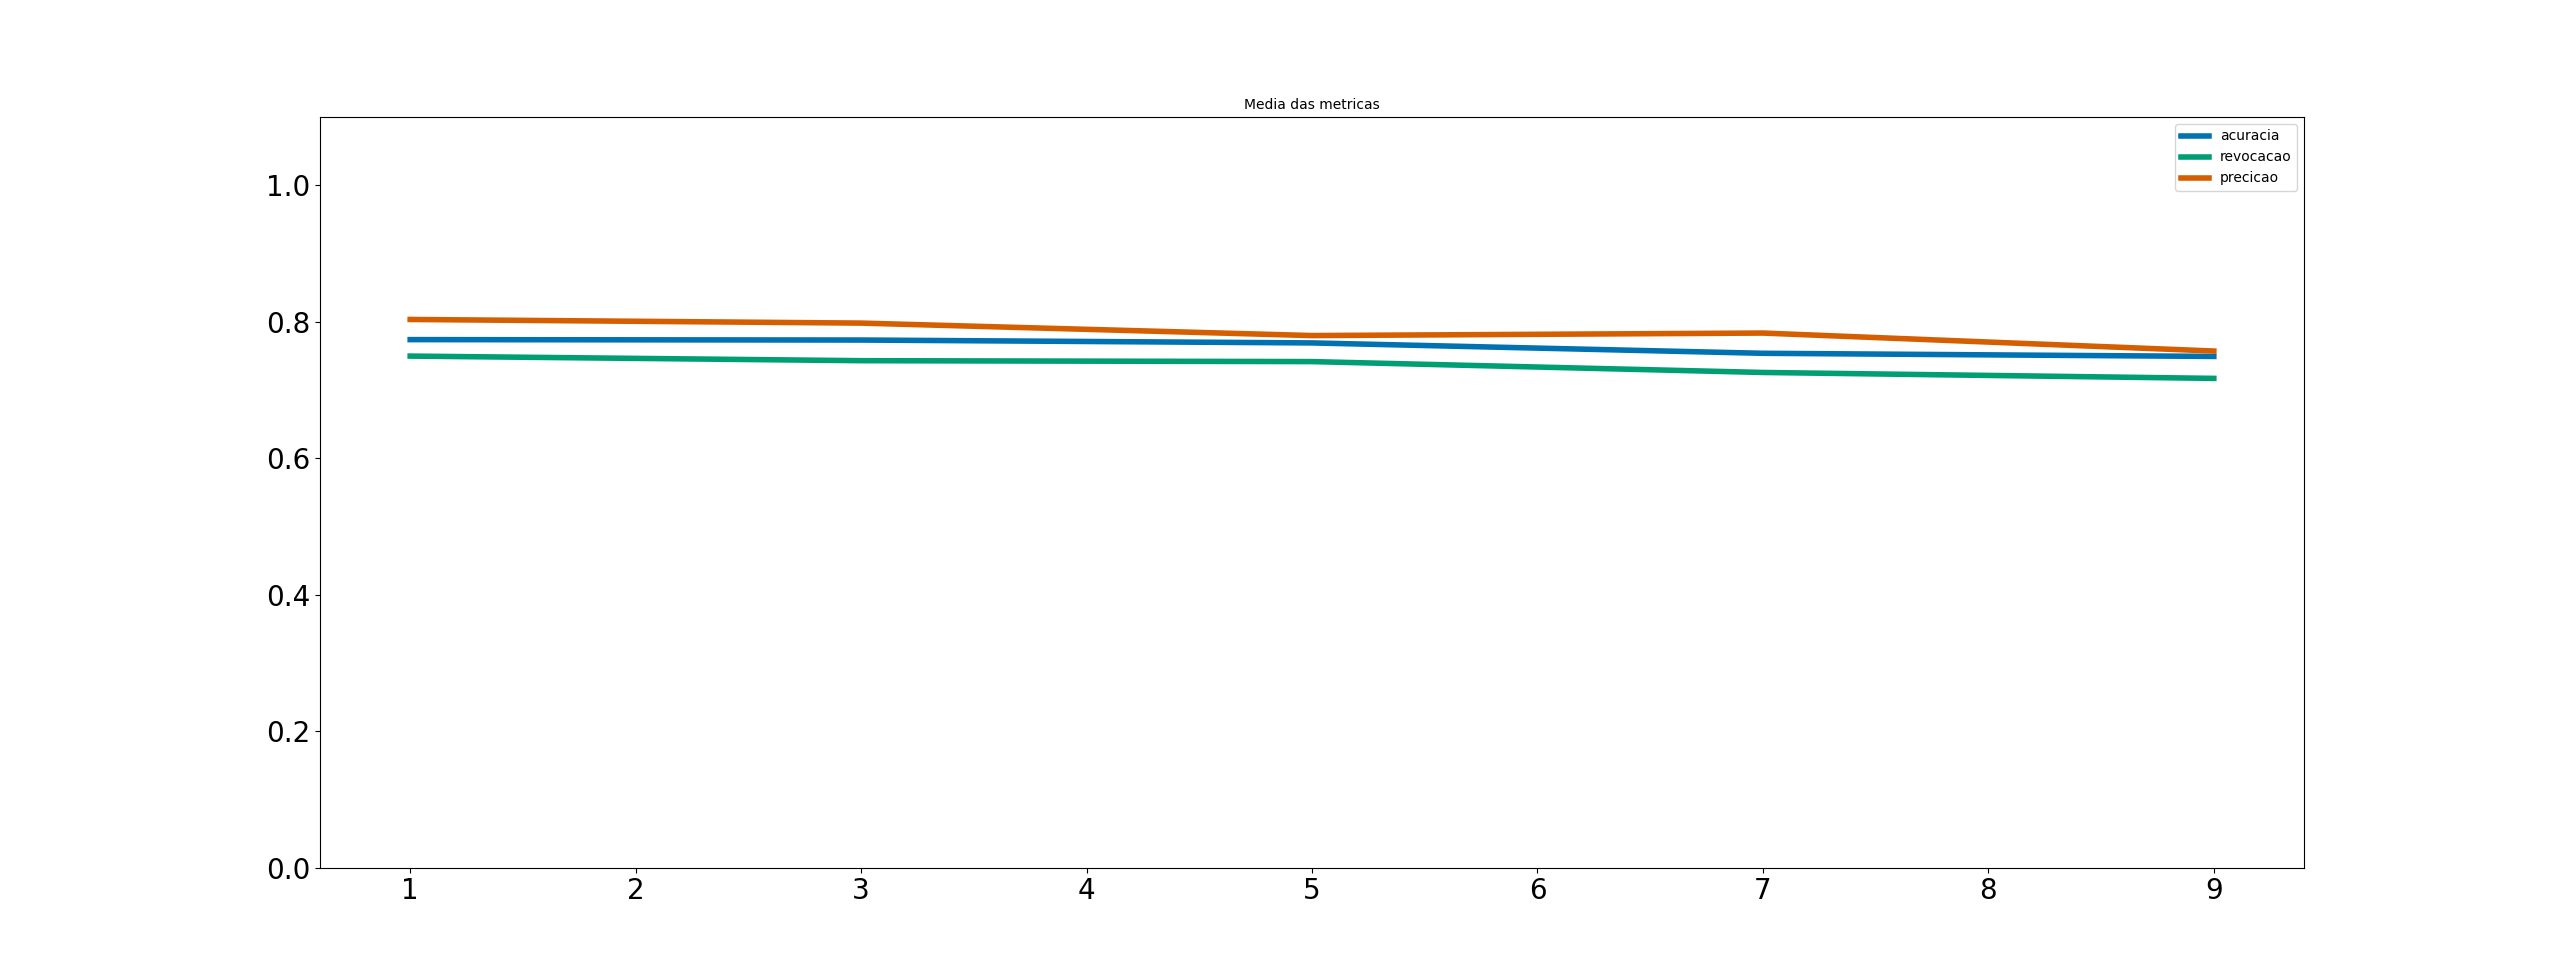
\includegraphics[width=\textwidth]{metricas.png}

Na figura acima, é possivel ver os resultados medios de todos os datasets. O resultando parece ser contraditorio com o apresentado individualmente, aonde o numero de vizinhos parece não afetar o resultado. Isso provalvemente está ocorrendo pelas oscilações negativas estarem cancelando as positivas.

O codigo que gerou essas imagens está disponivel no arquivo images.py

\end{document}